% Created by tikzDevice version 0.7.0 on 2015-04-25 18:17:40
% !TEX encoding = UTF-8 Unicode
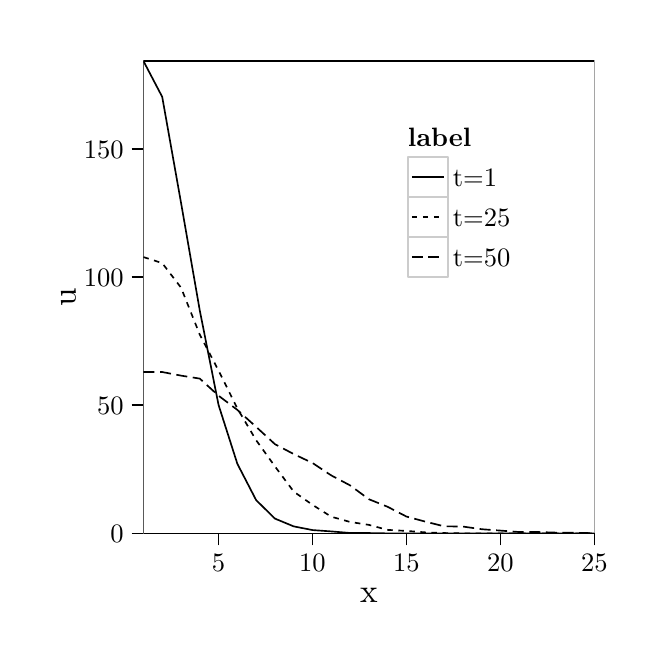
\begin{tikzpicture}[x=1pt,y=1pt]
\definecolor[named]{fillColor}{rgb}{1.00,1.00,1.00}
\path[use as bounding box,fill=fillColor,fill opacity=0.00] (0,0) rectangle (216.81,216.81);
\begin{scope}
\path[clip] (  0.00,  0.00) rectangle (216.81,216.81);
\definecolor[named]{drawColor}{rgb}{1.00,1.00,1.00}
\definecolor[named]{fillColor}{rgb}{1.00,1.00,1.00}

\path[draw=drawColor,line width= 0.6pt,line join=round,line cap=round,fill=fillColor] ( -0.00,  0.00) rectangle (216.81,216.81);
\end{scope}
\begin{scope}
\path[clip] ( 41.82, 34.03) rectangle (204.76,204.77);
\definecolor[named]{fillColor}{rgb}{1.00,1.00,1.00}

\path[fill=fillColor] ( 41.82, 34.03) rectangle (204.76,204.77);
\definecolor[named]{drawColor}{rgb}{0.00,0.00,0.00}

\path[draw=drawColor,line width= 0.6pt,line join=round] ( 41.82,204.77) --
	( 48.61,191.82) --
	( 55.40,153.62) --
	( 62.19,114.61) --
	( 68.98, 80.45) --
	( 75.77, 59.21) --
	( 82.56, 46.08) --
	( 89.35, 39.41) --
	( 96.13, 36.60) --
	(102.92, 35.27) --
	(109.71, 34.78) --
	(116.50, 34.22) --
	(123.29, 34.19) --
	(130.08, 34.07) --
	(136.87, 34.03) --
	(143.66, 34.03) --
	(150.45, 34.03) --
	(157.24, 34.03) --
	(164.03, 34.03) --
	(170.82, 34.03) --
	(177.61, 34.03) --
	(184.40, 34.03) --
	(191.19, 34.03) --
	(197.98, 34.03) --
	(204.76, 34.03);

\path[draw=drawColor,line width= 0.6pt,dash pattern=on 2pt off 2pt ,line join=round] ( 41.82,133.92) --
	( 48.61,131.75) --
	( 55.40,122.89) --
	( 62.19,105.90) --
	( 68.98, 92.87) --
	( 75.77, 79.22) --
	( 82.56, 67.73) --
	( 89.35, 58.28) --
	( 96.13, 49.17) --
	(102.92, 44.38) --
	(109.71, 40.09) --
	(116.50, 38.20) --
	(123.29, 37.15) --
	(130.08, 35.33) --
	(136.87, 34.96) --
	(143.66, 34.44) --
	(150.45, 34.19) --
	(157.24, 34.07) --
	(164.03, 34.03) --
	(170.82, 34.03) --
	(177.61, 34.03) --
	(184.40, 34.03) --
	(191.19, 34.03) --
	(197.98, 34.03) --
	(204.76, 34.03);

\path[draw=drawColor,line width= 0.6pt,dash pattern=on 4pt off 2pt ,line join=round] ( 41.82, 92.38) --
	( 48.61, 92.38) --
	( 55.40, 91.08) --
	( 62.19, 90.00) --
	( 68.98, 83.82) --
	( 75.77, 78.69) --
	( 82.56, 72.55) --
	( 89.35, 66.31) --
	( 96.13, 62.73) --
	(102.92, 59.51) --
	(109.71, 55.01) --
	(116.50, 51.42) --
	(123.29, 46.42) --
	(130.08, 43.67) --
	(136.87, 40.15) --
	(143.66, 38.33) --
	(150.45, 36.63) --
	(157.24, 36.54) --
	(164.03, 35.58) --
	(170.82, 35.08) --
	(177.61, 34.56) --
	(184.40, 34.56) --
	(191.19, 34.34) --
	(197.98, 34.28) --
	(204.76, 34.13);

\path[draw=drawColor,line width= 0.6pt,line join=round,line cap=round] ( 41.82, 34.03) rectangle (204.76,204.77);
\end{scope}
\begin{scope}
\path[clip] (  0.00,  0.00) rectangle (216.81,216.81);
\definecolor[named]{drawColor}{rgb}{0.00,0.00,0.00}

\node[text=drawColor,anchor=base east,inner sep=0pt, outer sep=0pt, scale=  0.96] at ( 34.71, 30.73) {0};

\node[text=drawColor,anchor=base east,inner sep=0pt, outer sep=0pt, scale=  0.96] at ( 34.71, 77.06) {50};

\node[text=drawColor,anchor=base east,inner sep=0pt, outer sep=0pt, scale=  0.96] at ( 34.71,123.38) {100};

\node[text=drawColor,anchor=base east,inner sep=0pt, outer sep=0pt, scale=  0.96] at ( 34.71,169.71) {150};
\end{scope}
\begin{scope}
\path[clip] (  0.00,  0.00) rectangle (216.81,216.81);
\definecolor[named]{drawColor}{rgb}{0.00,0.00,0.00}

\path[draw=drawColor,line width= 0.6pt,line join=round] ( 37.55, 34.03) --
	( 41.82, 34.03);

\path[draw=drawColor,line width= 0.6pt,line join=round] ( 37.55, 80.36) --
	( 41.82, 80.36);

\path[draw=drawColor,line width= 0.6pt,line join=round] ( 37.55,126.69) --
	( 41.82,126.69);

\path[draw=drawColor,line width= 0.6pt,line join=round] ( 37.55,173.02) --
	( 41.82,173.02);
\end{scope}
\begin{scope}
\path[clip] (  0.00,  0.00) rectangle (216.81,216.81);
\definecolor[named]{drawColor}{rgb}{0.00,0.00,0.00}

\path[draw=drawColor,line width= 0.6pt,line join=round] ( 68.98, 29.77) --
	( 68.98, 34.03);

\path[draw=drawColor,line width= 0.6pt,line join=round] (102.92, 29.77) --
	(102.92, 34.03);

\path[draw=drawColor,line width= 0.6pt,line join=round] (136.87, 29.77) --
	(136.87, 34.03);

\path[draw=drawColor,line width= 0.6pt,line join=round] (170.82, 29.77) --
	(170.82, 34.03);

\path[draw=drawColor,line width= 0.6pt,line join=round] (204.76, 29.77) --
	(204.76, 34.03);
\end{scope}
\begin{scope}
\path[clip] (  0.00,  0.00) rectangle (216.81,216.81);
\definecolor[named]{drawColor}{rgb}{0.00,0.00,0.00}

\node[text=drawColor,anchor=base,inner sep=0pt, outer sep=0pt, scale=  0.96] at ( 68.98, 20.31) {5};

\node[text=drawColor,anchor=base,inner sep=0pt, outer sep=0pt, scale=  0.96] at (102.92, 20.31) {10};

\node[text=drawColor,anchor=base,inner sep=0pt, outer sep=0pt, scale=  0.96] at (136.87, 20.31) {15};

\node[text=drawColor,anchor=base,inner sep=0pt, outer sep=0pt, scale=  0.96] at (170.82, 20.31) {20};

\node[text=drawColor,anchor=base,inner sep=0pt, outer sep=0pt, scale=  0.96] at (204.76, 20.31) {25};
\end{scope}
\begin{scope}
\path[clip] (  0.00,  0.00) rectangle (216.81,216.81);
\definecolor[named]{drawColor}{rgb}{0.00,0.00,0.00}

\node[text=drawColor,anchor=base,inner sep=0pt, outer sep=0pt, scale=  1.20] at (123.29,  9.03) {x};
\end{scope}
\begin{scope}
\path[clip] (  0.00,  0.00) rectangle (216.81,216.81);
\definecolor[named]{drawColor}{rgb}{0.00,0.00,0.00}

\node[text=drawColor,rotate= 90.00,anchor=base,inner sep=0pt, outer sep=0pt, scale=  1.20] at ( 17.30,119.40) {u};
\end{scope}
\begin{scope}
\path[clip] (  0.00,  0.00) rectangle (216.81,216.81);
\definecolor[named]{fillColor}{rgb}{1.00,1.00,1.00}

\path[fill=fillColor] (133.09,122.48) rectangle (178.68,184.61);
\end{scope}
\begin{scope}
\path[clip] (  0.00,  0.00) rectangle (216.81,216.81);
\definecolor[named]{drawColor}{rgb}{0.00,0.00,0.00}

\node[text=drawColor,anchor=base west,inner sep=0pt, outer sep=0pt, scale=  0.96] at (137.35,173.72) {\bfseries label};
\end{scope}
\begin{scope}
\path[clip] (  0.00,  0.00) rectangle (216.81,216.81);
\definecolor[named]{drawColor}{rgb}{0.80,0.80,0.80}
\definecolor[named]{fillColor}{rgb}{1.00,1.00,1.00}

\path[draw=drawColor,line width= 0.6pt,line join=round,line cap=round,fill=fillColor] (137.35,155.65) rectangle (151.81,170.11);
\end{scope}
\begin{scope}
\path[clip] (  0.00,  0.00) rectangle (216.81,216.81);
\definecolor[named]{drawColor}{rgb}{0.00,0.00,0.00}

\path[draw=drawColor,line width= 0.6pt,line join=round] (138.80,162.88) -- (150.36,162.88);
\end{scope}
\begin{scope}
\path[clip] (  0.00,  0.00) rectangle (216.81,216.81);
\definecolor[named]{drawColor}{rgb}{0.80,0.80,0.80}
\definecolor[named]{fillColor}{rgb}{1.00,1.00,1.00}

\path[draw=drawColor,line width= 0.6pt,line join=round,line cap=round,fill=fillColor] (137.35,141.20) rectangle (151.81,155.65);
\end{scope}
\begin{scope}
\path[clip] (  0.00,  0.00) rectangle (216.81,216.81);
\definecolor[named]{drawColor}{rgb}{0.00,0.00,0.00}

\path[draw=drawColor,line width= 0.6pt,dash pattern=on 2pt off 2pt ,line join=round] (138.80,148.43) -- (150.36,148.43);
\end{scope}
\begin{scope}
\path[clip] (  0.00,  0.00) rectangle (216.81,216.81);
\definecolor[named]{drawColor}{rgb}{0.80,0.80,0.80}
\definecolor[named]{fillColor}{rgb}{1.00,1.00,1.00}

\path[draw=drawColor,line width= 0.6pt,line join=round,line cap=round,fill=fillColor] (137.35,126.75) rectangle (151.81,141.20);
\end{scope}
\begin{scope}
\path[clip] (  0.00,  0.00) rectangle (216.81,216.81);
\definecolor[named]{drawColor}{rgb}{0.00,0.00,0.00}

\path[draw=drawColor,line width= 0.6pt,dash pattern=on 4pt off 2pt ,line join=round] (138.80,133.97) -- (150.36,133.97);
\end{scope}
\begin{scope}
\path[clip] (  0.00,  0.00) rectangle (216.81,216.81);
\definecolor[named]{drawColor}{rgb}{0.00,0.00,0.00}

\node[text=drawColor,anchor=base west,inner sep=0pt, outer sep=0pt, scale=  0.96] at (153.61,159.57) {t=1};
\end{scope}
\begin{scope}
\path[clip] (  0.00,  0.00) rectangle (216.81,216.81);
\definecolor[named]{drawColor}{rgb}{0.00,0.00,0.00}

\node[text=drawColor,anchor=base west,inner sep=0pt, outer sep=0pt, scale=  0.96] at (153.61,145.12) {t=25};
\end{scope}
\begin{scope}
\path[clip] (  0.00,  0.00) rectangle (216.81,216.81);
\definecolor[named]{drawColor}{rgb}{0.00,0.00,0.00}

\node[text=drawColor,anchor=base west,inner sep=0pt, outer sep=0pt, scale=  0.96] at (153.61,130.67) {t=50};
\end{scope}
\end{tikzpicture}
